\begin{figure}[htbp]
  \centering
    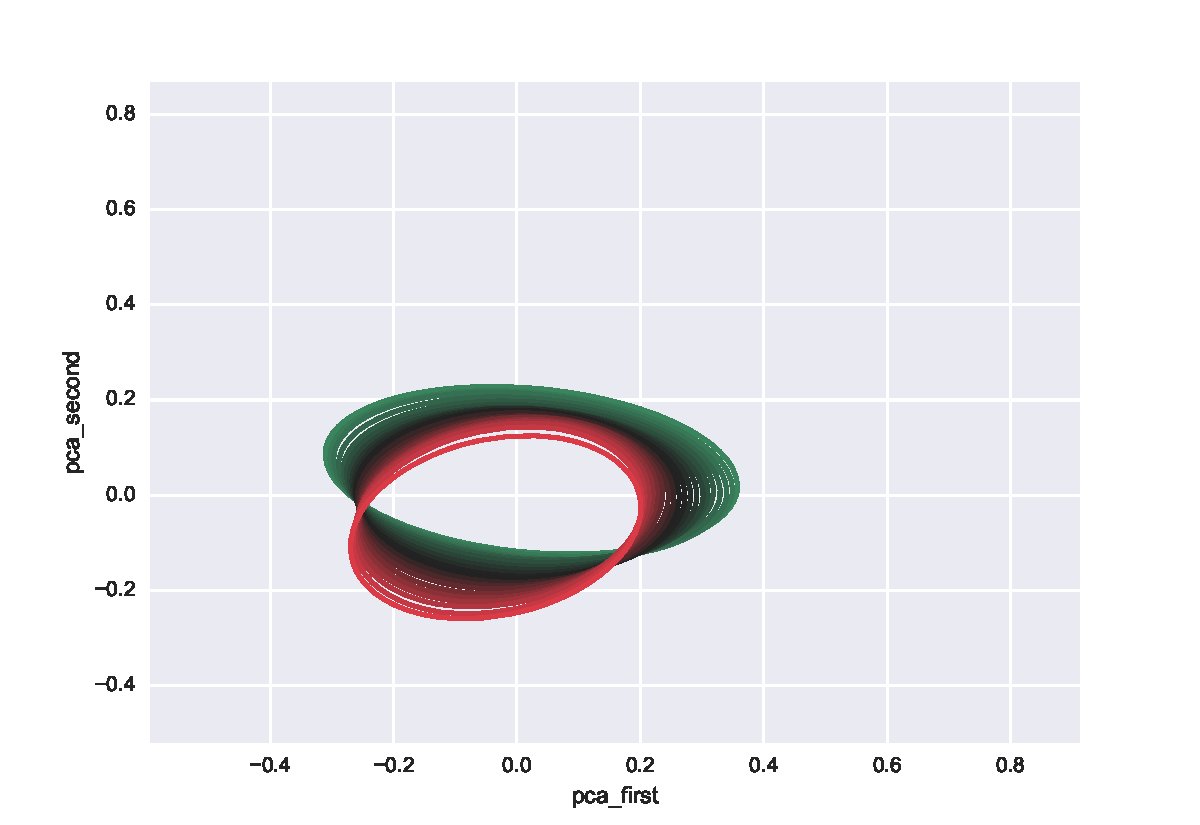
\includegraphics[clip,width=11.0cm]{fig/ellipse_pca_first_pca_second.pdf}
    \caption{主成分分析を行ったあとのデータ点から,各時刻ごとに二次元正規分布を求め,楕円としてプロットしたもの.楕円の大きさは,標準偏差の1倍になっている.緑から赤に近づくに連れて車線変更開始が近づいている.}
    \label{fig:pca_gauss}
\end{figure}
